\documentclass[conference]{IEEEtran}

%% \documentclass[sigconf]{acmart}

% The following packages can be found on http:\\www.ctan.org
\usepackage{tikz}     % For adding axes to plots
\usepackage{graphicx} % For including PDFs
\usetikzlibrary{positioning}
\usepackage{hyperref}


\usepackage{amsmath} % assumes amsmath package installed
\usepackage{amssymb}  % assumes amsmath package installed
\usepackage{textcomp} % For the text tilde low
\usepackage{tabularx}
    \newcolumntype{L}{>{\raggedright\arraybackslash}X}

%% Command for creating multiplie-line cells inside a table environment
\newcommand{\multilinecell}[2][c]{%
  \begin{tabular}[#1]{@{}c@{}}#2\end{tabular}}
  
%% Command for a text tilde
\newcommand{\thomastilde}{\raisebox{0.1ex}{\texttildelow}}

%% Make citations group together.
\usepackage[noadjust]{cite}

\begin{document}

\title{A Case Study on a Sustainable Framework for Ethically Aware Predictive Modeling}

\author{\IEEEauthorblockN{Anonymous Author(s)}}

%% \author{%
%%   \IEEEauthorblockN{Thomas Lux}%
%%   \IEEEauthorblockA{Department of Computer Science\\%
%%     Virginia Polytechnic Institute and State University\\%
%%     Blacksburg, Virginia 24060\\%
%%     Email: tchlux@vt.edu}%
%%   \and%
%%   \IEEEauthorblockN{Stefan Nagy}%
%%   \IEEEauthorblockA{Department of Computer Science\\%
%%     Virginia Polytechnic Institute and State University\\%
%%     Blacksburg, Virginia 24060}%
%%   \and%
%%   \IEEEauthorblockN{Mohammed Almanaa}%
%%   \IEEEauthorblockA{Department of Civil Engineering\\%
%%     Virginia Polytechnic Institute and State University\\%
%%     Blacksburg, Virginia 24060}%
%%   \and%
%%   \IEEEauthorblockN{Sirui Yao}%
%%   \IEEEauthorblockA{Department of Computer Science\\%
%%     Virginia Polytechnic Institute and State University\\%
%%     Blacksburg, Virginia 24060}%
%%   \and%
%%   \IEEEauthorblockN{Reid Bixler}%
%%   \IEEEauthorblockA{Department of Computer Science\\%
%%     Virginia Polytechnic Institute and State University\\%
%%     Blacksburg, Virginia 24060}%
%% }

% \thanks{$^{1}$ Student in Department of Civil Engineering}%
% \thanks{$^{2}$ Student in Department of Computer Science}%

% \thispagestyle{empty}
% \pagestyle{empty}

\maketitle

%% \IEEEpeerreviewmaketitle


%%%%%%%%%%%%%%%%%%%%%%%%%%%%%%%%%%%%%%%%%%%%%%%%%%%%%%%%%%%%%%%%%%%%%%%%%%%%%%%%
\begin{abstract}
Large volumes of data allow for modern application of statistical and mathematical models to practical social issues. Many applications of predictive models like criminal activity heatmapping, recidivism estimation, and child safety scoring rely on data that may be incomplete, incorrect, or biased. Many sensitive social and historical issues can unintentionally be incorporated into predictions causing ethical mistreatment. This work proposes a mechanism for continuously mitigating model bias by using algorithms that produce predictions from reasonably small sets of data, allowing a human-in-the-loop approach to model application. The benefits offered by this framework are twofold: (1) bias can be identified either statistically or by human users on a per-prediction basis; (2) data can be cleaned for bias on a per-prediction basis. A modeling and data management methodology similar to that presented here could strengthen the ethical application of data science and make the process of cleaning and validating data manageable in the long term.
\end{abstract}
%%%%%%%%%%%%%%%%%%%%%%%%%%%%%%%%%%%%%%%%%%%%%%%%%%%%%%%%%%%%%%%%%%%%%%%%%%%%%%%%
 
%% \IEEEkeywords{Ethics, Predictive Models, Multilayer Perceptron, Decision Tree, Local}


\section{INTRODUCTION}
\label{sec:introduction}
Data collection efforts are often aimed at providing or improving services for our communities and society as a whole. Large scale predictive models have coevolved with the explosion of available data since the start of the digital age and these models are practically necessary for success in domains as diverse as healthcare, employment, finance, and government. Creators of predictive models were motivated by a critical need to anticipate the future and to take action in advance. When the models succeed they can create life-saving value \cite{tomavsev2019clinically} or change economies \cite{siegel2016predictive}, but when they fail they can reinforce historical social injustice \cite{angwinmachine} and leave at-risk children without needed help \cite{eubanks2018child}. It is not surprising then that interpretability is an important research area for commonly used predictive models \cite{vellido2012making,doshi2018considerations,du2018techniques}.

A model is often considered unethical when it violates the expected practices and procedures of a formal agency like a government or business. For example, a model built from anonymous historical data and designed to assist a business in effective employee hiring may recover protected demographic information on the race, sex, or religion of the applicant. However, Title VII of United States federal code prohibits the use of this information in employment decisions. The predictive model would be acting unethically and unlawfully, but the user (the business) may be entirely unaware.

Many researchers have unveiled clear signs of unequal and racial treatment of individuals by predictive models \cite{squires2003racial,stoll2004black,angwinmachine}.  For example, Angwin et al. analyzed a well-known criminal risk assessment: COMPAS and concluded the outcomes of the model are racially biased \cite{angwinmachine}. They showed that ``Black defendants were twice as likely as white defendants to be misclassified as a higher risk of violent recidivism, and white recidivists were misclassified as low risk 63.2 percent more often than black defendants.'' The U.S. government has acknowledged the enormous potential for negative impact in biased models and the White House published several reports highlighting the potential bias that could adversely affect individuals or groups \cite{smith2016big}. Research is constantly underway that proposes ethical frameworks and potential solutions to protect principles of ethics and privacy \cite{dedeo2014wrong,vayena2016elements,kass2001ethics}.

In an effort to prevent biased and discriminatory decisions, policy makers and practitioners have classified unwanted discriminatory attributes as protected information that cannot be used as predictors in a model. However, a model made from anonymized unprotected data can become unethical even when it is not provided protected information. The model needs only to infer protected characteristics from the provided data in the prediction process \cite{dedeo2014wrong,pedreshi2008discrimination}. The possibility of protected inference makes developing unbiased models challenging, particularly when large amounts of data are involved. A burden is placed on users, who must identify ways to ensure predictions remain ethically sound. Generally there are only two methods to ensure a model is not violating ethical expectations: either carefully monitor and analyze all predictions for ethical mistreatment, or guarantee that the data utilized by the model (and how that data is used to predict) is ethically sound. This work makes an argument for the latter, as a common class of models can make good predictions from human-digestible amounts of data.

This paper makes an argument for per-prediction ethical validation of data and models via local approximation methods that produce interpretable results. The improvements offered by this methodology are twofold: (1) bias can be identified either statistically or by human users on a per-prediction basis; (2) data can be cleaned for bias on a per-prediction (regular) basis. Modeling techniques similar to those presented in this work could not only strengthen the ethical application of data science, but also make the process of cleaning and validating data manageable in the long term.


\section{RELATED WORK}
\label{sec:related}
Algorithmic bias has long been a subject of research on machine learning \cite{kirkpatrick2016battling, hajian2016algorithmic, baeza2016data}. 
Mitchell \cite{mitchell1980need} initially defined machine learning bias as ``any basis for choosing one generalization over another, other than strict consistency with the instances''.
Mooney \cite{mooney1996comparative} expanded this definition with the following assertions: (1) that every model bears some inherent bias, and (2) that detecting a model's bias requires comparison against others.
In recent years, the broad adoption of machine learning has made algorithmic bias a factor in real-world data discrimination \cite{squires2003racial, stoll2004black, angwinmachine}.

Several prior works have explored the problem of measuring algorithmic bias \cite{romei2014multidisciplinary, kamiran2013quantifying, zliobaite2015survey}.
Calders \& Verwer \cite{Calders2010} formalized discrimination as, given an input characteristic, the unequal distribution of outputs for different groups. 
Calders-Verwer (CV) scoring is frequently \cite{kamishima2011fairness, kamishima2012fairness, galhotra2017fairness, kamiran2012decision, vzliobaite2011handling} used to measure \emph{group discrimination} \cite{zafar2015learning, zemel2013learning}. For example, if a loan classifier produces dissimilar outcomes for both sexes (e.g. $P(Y=loan|S=male) > P(Y=loan|S=female)$), then its CV score is measured as the difference in outcomes between those groups (e.g. $P(Y=loan|S=male) - P(Y=loan|S=female)$.
Many works have since expanded on CV scoring for preventing discrimination \cite{zafar2017fairness, kamiran2013techniques, galhotra2017fairness}. 
Four general approaches exist: (1) \emph{Suppression} -- removing attributes most correlating with discrimination-sensitive attributes; (2) \emph{Dataset ``massaging''} -- altering labels of some objects to mitigate unwanted classifier outcomes; (3) \emph{Reweighting} -- assigning data carefully chosen weights to lessen the degree of discrimination; (4) \emph{Sampling} -- under- and over-sampling certain groups to compensate.

A recent focus of machine learning and data science research has been on improving model interpretability \cite{lipton2016mythos, juang2013data}. More specific goals include transparency for assessing model ethicality \cite{goodman2017european, herman2017data}, augmenting informativeness \cite{kim2015interactive, yang2018visually, wu2017interpretable}, and inferring causality \cite{syed2009enzyme}. An obstacle to model interpretability is the lack of transparency of black-box classifiers such as deep neural networks \cite{casillas2013interpretability, cortez2013using, krause2016interacting}.  Post-hoc interpretability \cite{lipton2016mythos} (e.g. visualizations or explanations) represents a promising alternative, however, formalizing  ``model-agnostic'' methodologies remains an ongoing research problem \cite{ribeiro2016should}.


\section{Model Descriptions}

In order to construct a predictive model from data, it is usually assumed that the phenomenon being predicted has some underlying \textit{function} that can be approximated. Many algorithms exist for constructing approximations of unknown functions given data. The following subsections roughly outline the mathematical formulation of both the (arguably more popular) \textit{global} models and the (less popular) \textit{local} models analyzed in the present case study.

\subsection{Global Predictive Models}
Classic machine learning and data science techniques applied today often rely on solving a very specific problem. They create a global predictive model with the aim of capturing trends that exist across (hundreds of) thousands of examples. In general, these global models are constructed given real valued data matrix $X \in \mathbb{R}^{n\ \times\ d}$, a truth function $f: \mathbb{R}^d \rightarrow \mathbb{R}$, and \textit{labels} $f(x^{(i)})$ for row vectors $x^{(i)} \in X$, $1 \leq i \leq n$. These models find the solution to

$$ \min_P \bigl\|\ \hat f_P(X) - f(X)\ \bigr\|, $$

\noindent where $\hat f_P: \mathbb{R}^d \rightarrow \mathbb{R}$ is the parametric approximation, $f(X)$ is used to denote the vector with components $f(X)_i = f(x^{(i)})$, and $\| \cdot \|$ is an appropriate measure. The labels may be real numbers, like probability of recidivism estimates, or categories such as ``safe'' or ``not safe'' for an at-risk child.

The difficulty with these models is that the minimization search which identifies the parameters for the model is performed over \textit{all} data. Whenever it is time to explain a prediction, the answer is often ``all data was used to capture this trend''. The models of this form that will be applied are a multilayer perceptron (MLP) and a decision tree (DT).

\subsubsection{Multilayer Perceptron}

The neural network is a well studied and widely used method for both regression and classification tasks \cite{hornik1989multilayer}. When using the rectified linear unit (ReLU) activation function \cite{dahl2013improving} and training with the BFGS minimization technique \cite{moller1993scaled}, the model built by a multilayer perceptron uses layers $l : \mathbb{R}^{i} \rightarrow \mathbb{R}^{j}$ defined by

$$ l(u) = \big( u^t W_l \big)_+ ,$$

\noindent where $W_l$ is the $i$ by $j$ weight matrix for layer $l$. In this form, the multilayer perceptron produces a piecewise linear model of the input data. The computational complexity of training a multilayer perceptron is $\mathcal{O}(n d m)$, where $m$ is determined by the sizes of the layers of the network and the stopping criterion of the BFGS minimization used for finding weights. This paper uses the scikit-learn MLP regressor \cite{scikit-learn}, a single hidden layer with 100 nodes, ReLU activation, and BFGS for training.

\subsubsection{Decision Tree}

The decision tree is used because of the relatively straightforward interpretation of the prediction process. Model construction is out of the scope of this description, but is a well-studied process \cite{quinlan1986induction}. A prediction at a point $z \in \mathbb{R}^d$ for a decision tree constructed over a real vector space is made by traversing nested axis-aligned conditionals of the form
$$\hat f(z) = \hat f(z | z_{k^{(1)}} \geq v^{(1)}, \ldots).$$

This paper uses the scikit-learn Decision Tree regressor \cite{scikit-learn}, no maximum depth or number of nodes, and the Gini impurity measure of information gain.

\subsection{Local Predictive Models}

The construction of approximation functions $\hat f_P: \mathbb{R}^d \rightarrow \mathbb{R}$ as described for global models can instead be approached on a per-prediction basis. A model is henceforth referred to as \textit{local} when any prediction made at a point $z \in \mathbb{R}^d$ is only a function of a set of points $L \subset X$, where membership in $L$ is determined by a distance metric. The advantage of using a local model is a more compact description of \textit{how} a prediction is made that is derived from a manageable subset of all known data. \textit{Local} models become particularly useful when predictions regard ethically sensitive issues and need to be rigorously evaluated for bias. The source data for any prediction can be checked on the spot for fairness of representation against any number of protected attributes.

The following sections describe the two local approximation techniques that will be used to predict recidivism likelihood in this work.

\subsubsection{Nearest Neighbor}

A well-studied technique for classification and approximation is the nearest neighbor algorithm \cite{cover1967nearest}. This algorithm (using the 2-norm to measure distance) will represent a baseline for comparison because it is the most mathematically simple \textit{local} model in this study. A prediction is made for Nearest Neighbor at point $z \in \mathbb{R}^d$ by
$$ \hat f(z) = f \big ( \text{\textit{argmin}}_{x^{(i)} \in X} \| z - x^{(i)} \|_2 \big). $$
This approximation technique can be applied in a wide range of applications, however it must be noted that the approximation surface it produces is not $C^0$ (continuous in value). An extension of this model that is not applied in this work, but could yield useful results is the $k$ nearest neighbor algorithm. This is further mentioned in Section \ref{sec:discussion}.

\subsubsection{Voronoi Mesh}

While nearest neighbor inherently utilizes the convex region $v^{x^{(i)}}$ (Voronoi cell \cite{dirichlet1850reduction}) consisting of all points closer to $x^{(i)}$ than any other point $x^{(j)}$. The Voronoi mesh \cite{lux2018novel} smooths the nearest neighbor approximation by utilizing the Voronoi cells to define support via a generic basis function $V: \mathbb{R}^d \rightarrow \mathbb{R}_+$ given by

$$ V^{x^{(i)}}(y) = \left(1 - \frac{\bigl\|y - x^{(i)}\bigr\|_2}{2 \ d(y \mid x^{(i)})} \right)_+, $$
where $x^{(i)}$ is the center of the Voronoi cell, $y \in \mathbb{R}^d$ is an interpolation point, and $d(y \mid x^{(i)})$ is the distance between $x^{(i)}$ and the boundary of the Voronoi cell $v^{x^{(i)}}$ in the direction $y - x^{(i)}$. $V^{x^{(i)}}\bigl(x^{(j)}\bigr) = \delta_{ij}$ and $V^{x^{(i)}}$ has local support. While $V^{x^{(i)}}(x^{(i)}) = 1$, the $2$ in the denominator causes all basis functions to go linearly to $0$ at the boundary of the twice-expanded Voronoi cell. Note that this basis function is $C^0$ because the boundaries of the Voronoi cell are $C^0$. In the case that there is no boundary along the vector $w$, the basis function value is always $1$.

While the cost of computing the exact Voronoi cells for any given set of points grows exponentially \cite{dutour2009complexity}, the calculation of $d$ is linear with respect to the number of control points and dimensions. Given any center $x^{(i)} \in \mathbb{R}^d$, set of control points $C \subseteq X$, and interpolation point $y \in \mathbb{R}^d$, $d\bigl(y \mid x^{(i)}\bigr)$ is the solution to
$$
  \max_{c \in C\backslash\{x^{(i)}\}} \frac{\bigl\|y - x^{(i)}\bigr\|_2}{2} \ \frac{y \cdot \bigl(c - x^{(i)}\bigr) - x^{(i)} \cdot \bigl(c - x^{(i)}\bigr)}{c \cdot \bigl(c - x^{(i)}\bigr) - x^{(i)} \cdot \bigl(c - x^{(i)}\bigr)}.
$$

The resulting algorithm is capable of producing predictions in $\mathcal{O}(n^2 d)$ computation time, which is relatively fast for all but tens of millions of points. Most importantly there is no \textit{training} for this algorithm, so as data is updated the fundamental model itself is changed accordingly.

%% ===================================================================


\begin{table*}
\begin{center}
\begin{tabular}{ c | c }
 \hline
 \textbf{FEATURE NAME} & \textbf{VALUES} \\
 \hline
 Sex & F, M \\
  \hline
 Age At Release & Under 25, 25-34, 35-44, 45-54, 55 and Older \\  
  \hline
 Convicting Offense Classification & Aggravated Misdemeanor, Serious Misdemeanor, Sexual Predator Community Supervision, etc \\
  \hline
Convicting Offense Subtype & Murder, Alcohol, Weapons, Drug Possession, Assault, Traffic, Burglary, Forgery/Fraud, Animals, Theft, etc\\  
 \hline
Release Type & Special Sentence, Parole Granted, Discharged - Expiration of Sentence, Released to Special Sentence, etc \\  
 \hline
Main Supervising District & 1JD, 2JD, 3JD, 4JD, 5JD, etc\\  
 \hline
Race -- Ethnicity & White (non-Hispanic), Black or African American, White (Hispanic), American Indian or Alaskan\\
 \hline
\end{tabular}
\end{center}
\caption{This table provides a sample of the values for features relevant to the recidivism prediction task.}
\label{table:1}
\end{table*}


\section{DATA AND RESULTS}
\label{sec:data}

A case study is presented to demonstrate the comparative performance of \textit{local} models versus \textit{global} models on an ethically sensitive prediction task. The comparison rests on a 3-Year Recidivism for Offenders Released from Prison in Iowa dataset, publicly available on the U.S. Government open data (\href{https://www.data.gov}{data.gov}) website. This dataset reports whether or not an offender is convicted of another crime within three years of being released from prison. This dataset naively provides a classification task (predict whether or not a released offender would recidivate) or, as will be considered here, it also provides a regression task (predict the probability of recidivism). By collapsing all entries with identical predictor values, this work converts each offender description into a collection of matching individuals with a single real-valued estimate for the probability of recidivism.

This dataset provides $21,646$ instances, among which $14,619$ instances do not recidivate and $7,027$ instances do recidivate. The distribution of ethnicities in this data are distinctly different from the ethnic distribution for the actual population of Iowa in 2016 (See Figure \ref{fig:mesh1}). There exists obvious gaps especially for White non-Hispanic ($67.4\%$ in data \textit{decreased} from $88.7\%$ of actual population) and Black or African American ($23.6\%$ in data \textit{increased} from  $2.9\%$ of actual population). 

\begin{figure}
  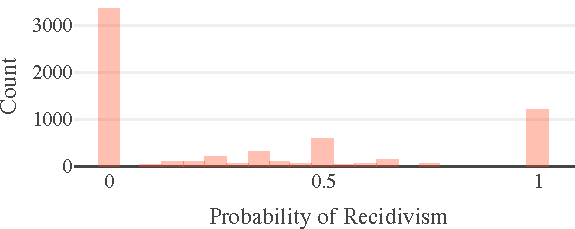
\includegraphics[width=.48\textwidth]{regression_values_histogram.pdf}
  \caption{A 20-bin histogram of the values for recidivism likelihood in the regression task composed of 6,632 samples.}
  \label{fig:histogram_of_recidivism}
\end{figure}

\begin{figure}
    \centering
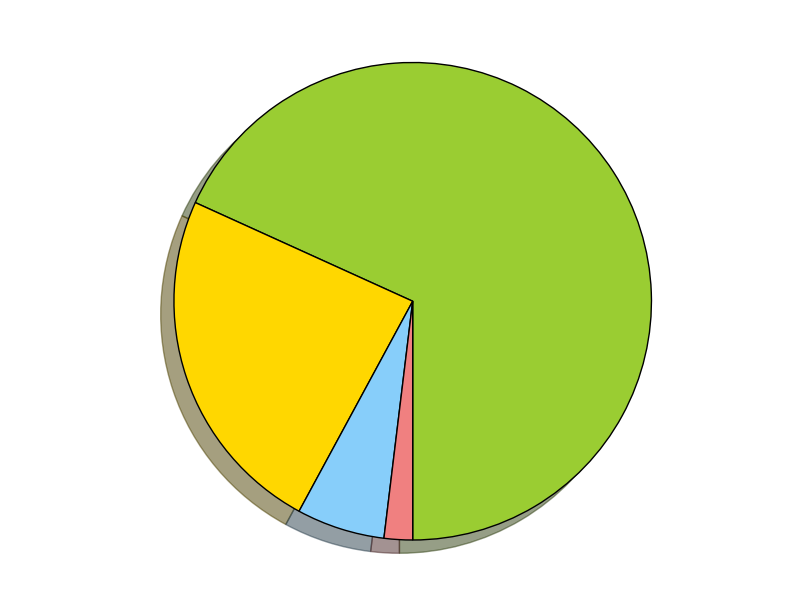
\includegraphics[scale=0.2]{figure_2.png}
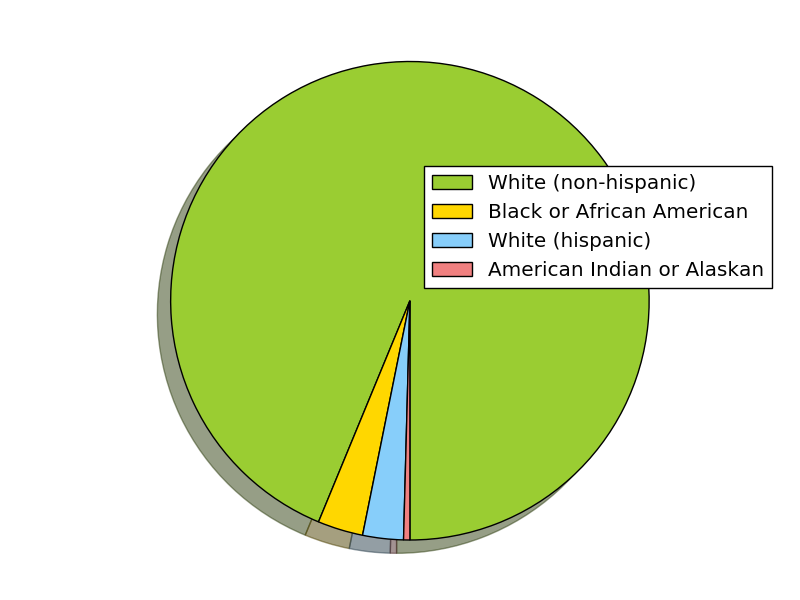
\includegraphics[scale=0.2]{figure_1.png}
    \caption{The distribution across ethnicity groups of the dataset (left) and the actual population in Iowa (right)}
    \label{fig:mesh1}
\end{figure}


The data provides 17 unique pieces of information related to each individual, including the crime committed in the case of recidivism (blank for non-recidivating individuals). The relevant features to this prediction task can be observed in Table \ref{table:1}. The omitted features are either not relevant to the prediction task, or are uniquely determined by one of the chosen features. For this work the ``Race -- Ethnicity'' is reserved as protected attribute (not available to models) and is later used to evaluate bias in predictions. Any categories with fewer than 100 samples are discarded in order to reduce the resulting dimension and prevent predictions from being made with statistically insignificant amounts of supporting data. Categorical features are encoded with $c$ unique categories into $\mathbb{R}^{c-1}$ by mapping each category onto one of the vertices of a regular simplex centered at 0 where all vertices $v$ satisfy $\|v\|_2 = 1$. The feature named ``Age At Release'' was tested as both the mean age of the range and as a mapped categorical. Results demonstrated insignificant differences in outcome, so the numerical mean age is used for experiments.

In all experiments, predictions are evaluated against the labeled recidivism probability while the race \& ethnicity information is used to evaluate model bias. After preprocessing, the original $21,018$ instances with $17$ features are reduced to $6,632$ in a $50$ dimensional real vector space. The distribution of recidivism probabilities can be seen in Figure \ref{fig:histogram_of_recidivism}.

In order to estimate the performance of the different algorithms, \textit{k-fold} cross validation as described in \cite{kohavi1995study} with $k=10$ is used. All algorithms are given the same ten folds of randomized training and testing data in order to maintain comparative fairness. Note that in this scheme there will be exactly one prediction made for each data point, meaning all analysis of results is done with the same sized data as described in Section \ref{sec:data}.

Figure \ref{fig:regression_performance} displays the evaluation of all algorithms. The Voronoi Mesh and Neural Network produce the best results. The prediction outcomes are promising, demonstrating that 50\% of recidivism likelihood predictions have less than a $16\%$ absolute error without any attempt at problem-specific tuning.


%% ===================================================================

\section{DISCUSSION}
\label{sec:discussion}

As can be observed in Figure \ref{fig:regression_performance}, the Voronoi Mesh (VM) algorithm can make a prediction based on roughly $2d$ (\thomastilde{}100) points from data and compete with the global fitting MLP that uses all data (\thomastilde{}7K) points. This demonstrates that local predictive models are capable of producing equally accurate predictions when compared with global predictive models with far more compact support from data.

The benefit of using the VM (or any local model) to make predictions in ethically sensitive applications is that \textit{every} prediction has a manageable set of source data that describes how a prediction is produced. Addressing the two points in Section \ref{sec:introduction}, statistical tests can be run on these source data points to reduce prediction bias in desirable ways (e.g. data could be filtered until the predictive population matches the demographics of the state). Human-readable source for a prediction also opens the door to regular validation of source data, an important aspect of model maintenance.

In order to maintain ethical conscientiousness in predictive modeling, it is vital that predictions can be audited for fairness and adherence to standards. Local predictive models provide a meaningful avenue for pursing the legal right to a representative sample, and the legal right to a fair prediction.

This case study provides only a glimpse at the prospective application of local models. There are far more advanced (and potentially more accurate models) with very similar properties: Delaunay triangulations (simplicial meshes) \cite{chang2018polynomial}, $k$ nearest neighbor, Linear Shepard \cite{thacker2010algorithm} (and other Shepard methods), and Box Spline Meshes \cite{lux2018novel}, name only a few.

% Almost all machine learning algorithms can be treated local models in which we use solely a fixed-length moving time window for training. This step would make the computational time smaller, giving us a great chance to apply it on online complex problems that cannot handle any delay in the prediction. Yet, this approach would not be ideal if there is a core knowledge that cannot be discovered without running the entire dataset.

% One must also note that the Asian or Pacific Islander category was also the smallest population size by far, meaning that having the highest percentage of bias from false positives is expected for all 4 models.



\begin{figure*}
\centering
\begin{tabular}{l r}

  % NearestNeighbor
  \begin{tabular}{c c}
    \vspace{3mm} \\
    \multicolumn{2}{c}{\textit{NearestNeighbor}} \\
    \multicolumn{2}{c}{ 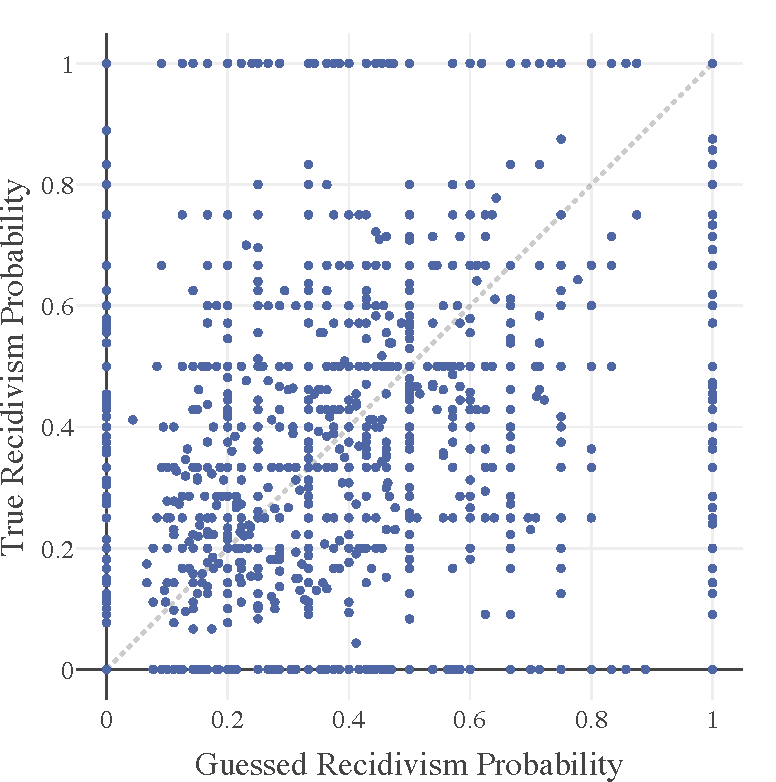
\includegraphics[width=2in,height=2in]{NearestNeighbor_regression.pdf}} \vspace{3mm} \\
    \begin{tabular}{c|c}
        Min & 0.000 \\
        $25^{th}$ & 0.033 \\
        $50^{th}$ & 0.167 \\
        $75^{th}$ & 0.400 \\
        Max & 1.000 \\
    \end{tabular} &
    \begin{tabular}{|c l|}
      \hline
      0.226 & White - NH \\
      0.250 & Black - NH \\
      0.200 & White - H \\
      0.167 & AI or NA \\
      0.306 & Asian or PI \\
      \hline
    \end{tabular} \vspace{3mm} \\
  \end{tabular}

  &

  % VoronoiMesh
  \begin{tabular}{c c}
    \vspace{3mm} \\
    \multicolumn{2}{c}{\textit{VoronoiMesh}} \\
    \multicolumn{2}{c}{ 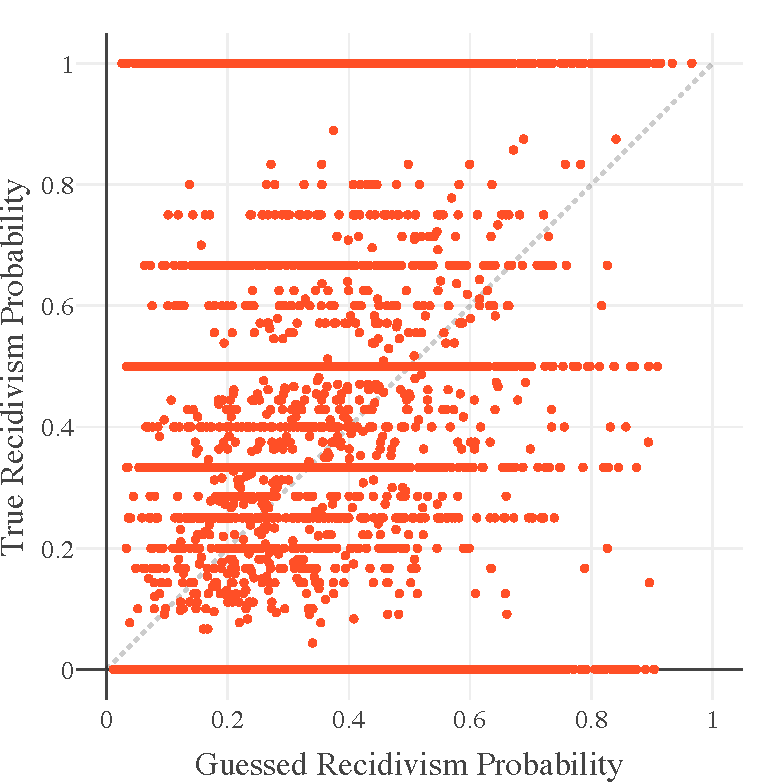
\includegraphics[width=2in,height=2in]{VoronoiMesh_regression.pdf}} \vspace{3mm} \\
    \begin{tabular}{c|c}
        Min & 0.000 \\
        $25^{th}$ & 0.072 \\
        $50^{th}$ & 0.156 \\
        $75^{th}$ & 0.291 \\
        Max & 0.974 \\
    \end{tabular} &
    \begin{tabular}{|c l|}
      \hline
      0.148 & White - NH \\
      0.161 & Black - NH \\
      0.125 & White - H \\
      0.129 & AI or NA \\
      0.139 & Asian or PI \\
      \hline
    \end{tabular} \vspace{3mm} \\
  \end{tabular}

  \\

  % DecisionTreeRegressor
  \begin{tabular}{c c}
    \vspace{3mm} \\
    \multicolumn{2}{c}{\textit{DecisionTreeRegressor}} \\
    \multicolumn{2}{c}{ 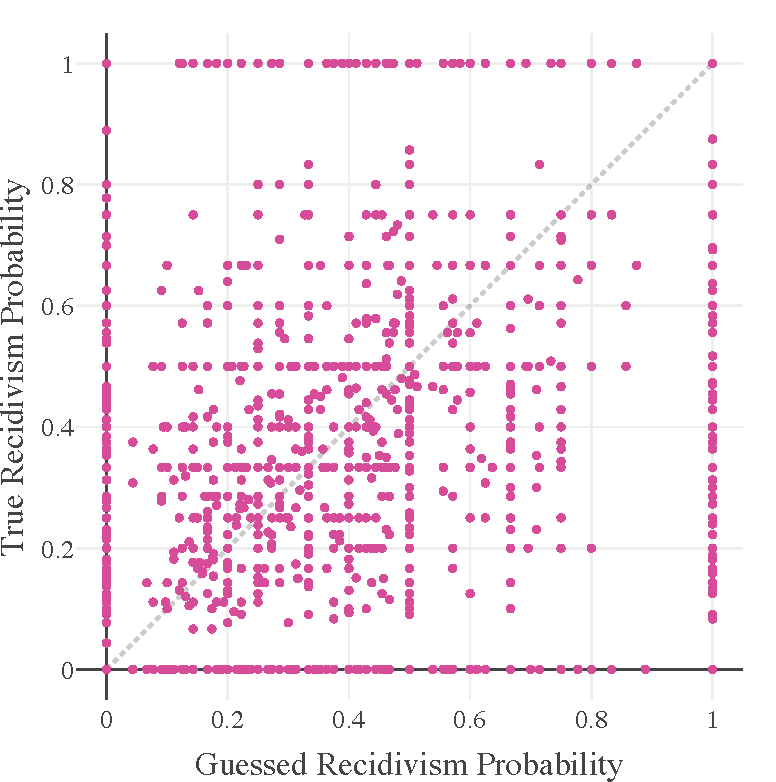
\includegraphics[width=2in,height=2in]{DecisionTreeRegressor_regression.pdf}} \vspace{3mm} \\
    \begin{tabular}{c|c}
        Min & 0.000 \\
        $25^{th}$ & 0.040 \\
        $50^{th}$ & 0.187 \\
        $75^{th}$ & 0.433 \\
        Max & 1.000 \\
    \end{tabular} &
    \begin{tabular}{|c l|}
      \hline
      0.250 & White - NH \\
      0.286 & Black - NH \\
      0.246 & White - H \\
      0.264 & AI or NA \\
      0.257 & Asian or PI \\
      \hline
    \end{tabular} \vspace{3mm} \\
  \end{tabular}

  &

  % MLPRegressor
  \begin{tabular}{c c}
    \vspace{3mm} \\
    \multicolumn{2}{c}{\textit{MLPRegressor}} \\
    \multicolumn{2}{c}{ 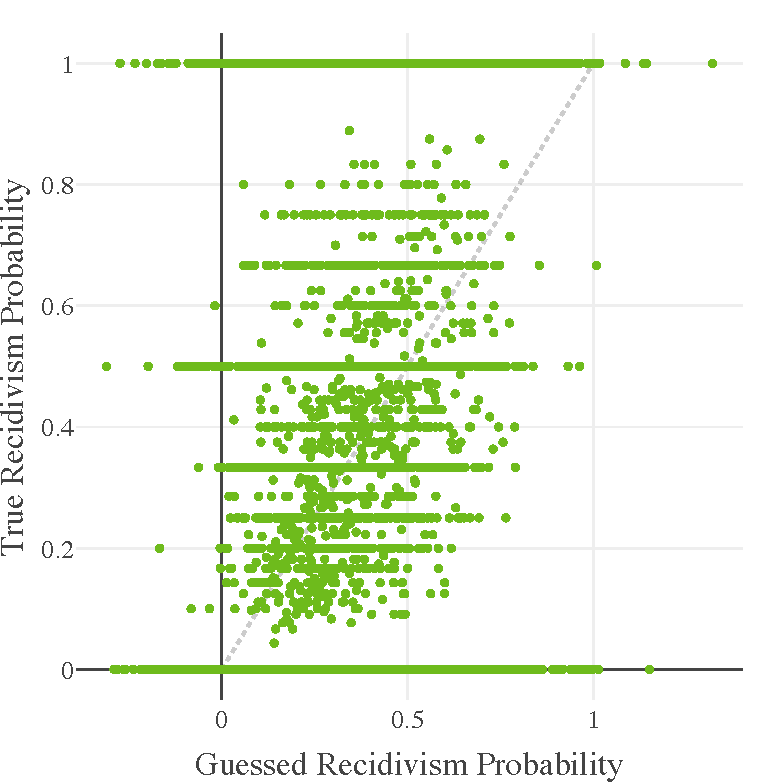
\includegraphics[width=2in,height=2in]{MLPRegressor_regression.pdf}} \vspace{3mm} \\
    \begin{tabular}{c|c}
        Min & 0.000 \\
        $25^{th}$ & 0.068 \\
        $50^{th}$ & 0.145 \\
        $75^{th}$ & 0.279 \\
        Max & 1.273 \\
    \end{tabular} &
    \begin{tabular}{|c l|}
      \hline
      0.147 & White - NH \\
      0.153 & Black - NH \\
      0.134 & White - H \\
      0.113 & AI or NA \\
      0.114 & Asian or PI \\
      \hline
    \end{tabular} \vspace{3mm} \\
  \end{tabular}

\end{tabular}

  \caption{These four plots show the true recidivism probability versus guessed recidivism probability for each of the regression techniques. The top two regression algorithms make predictions based only on local data while the bottom two algorithms are global fitting techniques. The left vertical table beneath each figure displays the percentiles of absolute errors when predicting the probability of recidivism with that algorithm. The right table beneath each figure shows the median error in recidivism likelihood for those predictions which were over-estimated (false positives) broken down by race. Notice that without additional constraints, the neural network produces predictions outside of the range [0,1].}
  \label{fig:regression_performance}
\end{figure*}


%% ===================================================================

\section{CONCLUSION}
\label{sec:conclusion}

This paper presents an argument for the application of local models to ethically sensitive prediction tasks. Sample results demonstrate that algorithms which rely only on local support are capable of producing predictions of comparable accuracy to popular global techniques while maintaining an enhanced level of predictive transparency. The potential for operating under more concise legal definitions and meaningful statistical analyses further supports the implementation of local prediction methodologies. A recidivism case study demonstrates that the use of more human-interpretable models for prediction could not only strengthen the ethical application of data science, but also make the process of cleaning and validating data manageable in the long term.

%% ===================================================================

\bibliographystyle{IEEEtran}
\bibliography{paper}

\end{document}
